\documentclass[prd,aps,twocolumn,floatfix,nofootinbib,superscriptaddress]{revtex4-2}

\usepackage{amsmath,amssymb}
\usepackage{graphicx}
\usepackage{booktabs}
\usepackage{xcolor}
\usepackage{hyperref}

\newcommand{\Mc}{M_{c}}
\newcommand{\Thawk}{T_{H}}
\newcommand{\GN}{G_{N}^{\rm emerg}}
\newcommand{\aADW}{\alpha_{\rm ADW}}
\newcommand{\Ladw}{\Lambda_{\rm UV}}
\newcommand{\Nf}{N_{f}}
\newcommand{\xivest}{\chi_{\rm vest}}
\newcommand{\dADW}{\delta_{\rm ADW}}

% Auto-generated by update_counts.py — 2026-11-05T17:29:00.839938
% Do not edit manually. Run: uv run python scripts/update_counts.py
\newcommand{\leantoolchain}{4.32.0}
\newcommand{\mathlibrev}{81a5d257}
\newcommand{\physlibrev}{c4843367}
\newcommand{\totaltheorems}{30948}
\newcommand{\substantivetheorems}{30922}
\newcommand{\placeholdertheorems}{26}
\newcommand{\kernelsubstantivetheorems}{30853}
\newcommand{\trackedvacuitydebt}{69}
\newcommand{\axiomcount}{0}
\newcommand{\sorrycount}{0}
\newcommand{\sorrypercent}{0.0}
\newcommand{\leanmodules}{2152}
\newcommand{\leandefinitions}{15467}
\newcommand{\pythonmodules}{140}
\newcommand{\testfiles}{218}
\newcommand{\totaltests}{8140}
\newcommand{\figurecount}{170}
\newcommand{\notebookcount}{91}
\newcommand{\papercount}{42}
\newcommand{\aristotleproved}{313}
\newcommand{\aristotleruns}{40}
% --- D11 bundle substrate summary (source-level, stated rule) ---
\newcommand{\dxiModules}{22}
\newcommand{\dxiLines}{6267}
\newcommand{\dxiTheorems}{403}
\newcommand{\dxiDefs}{82}
\newcommand{\dxiDepsTheorems}{409}
% --- Paper 18 / Phase 5t per-section counts (FermiHubbardDimer.lean) ---
\newcommand{\fhdTotal}{130}
\newcommand{\fhdWaveTwo}{13}
\newcommand{\fhdWaveThree}{6}
\newcommand{\fhdWaveFour}{19}
\newcommand{\fhdWaveFive}{20}
\newcommand{\fhdWaveSixABC}{35}
\newcommand{\fhdWaveSixExtra}{13}
\newcommand{\fhdWaveSeven}{17}
\newcommand{\fhdWaveEight}{7}
% --- Paper 26 / 27 per-module counts (BH entropy + four laws) ---
\newcommand{\bhEntropyTotal}{32}
\newcommand{\bhThermoTotal}{20}
% --- Phase 6 per-module + pytest counts (paper32 / paper34-38 / note_rt_ch_bounds) ---
\newcommand{\strongCpDeThms}{8}
\newcommand{\strongCpDeTests}{14}
\newcommand{\epThms}{24}
\newcommand{\epTests}{38}
\newcommand{\qecHolographyThms}{10}
\newcommand{\qecHolographyTests}{30}
\newcommand{\centerSymmThms}{18}
\newcommand{\centerSymmTests}{28}
\newcommand{\chiralSsbThms}{10}
\newcommand{\chiralSsbTests}{14}
\newcommand{\cflThms}{12}
\newcommand{\cflTests}{17}
\newcommand{\rtChThms}{7}
\newcommand{\rtChTests}{29}
\newcommand{\heatKernelThms}{20}
\newcommand{\heatKernelTests}{39}
\newcommand{\higherCurvatureThms}{13}
\newcommand{\higherCurvatureTests}{42}
\newcommand{\diffInvarianceThms}{13}
\newcommand{\diffInvarianceTests}{36}
\newcommand{\nonlinearEFEThms}{13}
\newcommand{\nonlinearEFETests}{40}
\newcommand{\microscopicCoefficientMatchThms}{12}
\newcommand{\microscopicCoefficientMatchTests}{42}
\newcommand{\einsteinCartanExtensionThms}{12}
\newcommand{\einsteinCartanExtensionTests}{41}
\newcommand{\bbnThms}{14}
\newcommand{\bbnTests}{16}
% --- Phase 6f/6g classical-GR per-module + wave totals (I1 §11–§13) ---
\newcommand{\curvatureThms}{14}
\newcommand{\einsteinTensorThms}{9}
\newcommand{\energyConditionsThms}{8}
\newcommand{\exactSolutionsThms}{16}
\newcommand{\admFormalismThms}{10}
\newcommand{\tetradFormalismThms}{5}
\newcommand{\phaseSixfWonesixTotal}{62}
\newcommand{\phaseSixfWsevenTotal}{13}
\newcommand{\riemannCoordinateThms}{8}
\newcommand{\riemannDifferentialBianchiThms}{8}
\newcommand{\bundleRiemannAuxThms}{6}
\newcommand{\bundleRiemannThms}{7}
\newcommand{\leviCivitaThms}{7}
\newcommand{\phaseSixfWeightTotal}{36}
\newcommand{\riccatiComparisonThms}{11}
\newcommand{\mazurSigmaModelRigidityThms}{12}
\newcommand{\hawkingPenroseCurveThms}{6}
\newcommand{\areaTheoremCurveThms}{10}
\newcommand{\phaseSixgWnineTotal}{39}
% --- D2 chirality-bundle per-module theorem counts (same convention as \totaltheorems) ---
\newcommand{\dtwoSmFermionDataThms}{19}
\newcommand{\dtwoZsixteenAnomalyThms}{23}
\newcommand{\dtwoVecGMonoidalThms}{11}
\newcommand{\dtwoToricCodeCenterThms}{25}
\newcommand{\dtwoCenterEquivalenceThms}{10}
\newcommand{\dtwoGoltermanShamirThms}{32}
\newcommand{\dtwoLatticeHamiltonianThms}{33}
\newcommand{\dtwoTpfEvasionThms}{14}
\newcommand{\dtwoPauliMatricesThms}{15}
\newcommand{\dtwoBdgHamiltonianThms}{8}
\newcommand{\dtwoChiralityWallMasterThms}{16}
\newcommand{\dtwoOnsagerAlgebraThms}{41}
\newcommand{\dtwoOnsagerContractionThms}{12}
\newcommand{\dtwoGtWeylDoubletThms}{15}
\newcommand{\dtwoFkGappedInterfaceThms}{12}
% --- paper10 per-module theorem counts (same convention as \totaltheorems) ---
\newcommand{\paperTenWangBridgeThms}{8}
\newcommand{\paperTenModularInvarianceThms}{11}
% --- Cross-platform Lean theorem reuse, 1+1D BEC -> 2+1D graphene (D1) ---
% Owner: scripts/count_theorem_reuse.py (population = the nine
% 1+1D BEC modules; REUSED = statement is platform-parametric).
\newcommand{\reuseTransferred}{107}
\newcommand{\reusePopulation}{120}
\newcommand{\reuseSpecific}{13}
\newcommand{\reusePercent}{89.17}
\newcommand{\reusePercentRounded}{89}
\newcommand{\reuseSpecificPercentRounded}{11}


\begin{document}

\title{BCH four laws and the regime partition for emergent-gravity ADW
black holes: a sign-of-$d\Thawk/dt$ partition between Schwarzschild
and acoustic evaporation}

\author{John G. Roehm}
\affiliation{SK-EFT Hawking Project (Phase 6a Wave 5)}

\date{\today}

\begin{abstract}
We formalize conditional mechanics constraints and local temperature
profiles for two proposed regimes of an emergent-gravity ADW substrate,
separated by a model critical mass $\Mc(\aADW, \Ladw, \Nf)$.
Above $\Mc$, the supplied Schwarzschild profile
follows the textbook Schwarzschild signature: $\Thawk = \hbar/(8\pi M)$
(Hawking 1975~\cite{Hawking1975CMP}), so during evaporation
$dM/dt < 0$ and $d\Thawk/dt > 0$ (heats as evaporates), with
finite evaporation time $t_{\rm evap} \sim M^3$ for that evolution.
The proposed branch below $\Mc$ uses the local cooling profile of
Balbinot, Fagnocchi and Fabbri~\cite{Balbinot2005PRD} as motivation:
$\Thawk(t) = (\hbar c / 2\pi) \kappa [1 - (563/720\pi)\,\varepsilon\, \kappa^3 c
A_0 t]$ in a constant-sound-speed nozzle. Their $t \sim 1/T^3$
late-time discussion is an extrapolation. It does not establish an
ADW evaporation endpoint or physical selection of the branch below
$\Mc$. The classifier transports supplied signs; a separate profile
criterion derives opposite local derivatives under explicit trajectory
and short-time assumptions. The full physical four laws and the
microscopic matching of the two branches remain required constructions. The substrate-response
coefficient ansatz $\dADW = (\aADW - 1)\Ladw$ vanishes in the bare
Sakharov--Adler limit and provides four falsifiability tests for any
candidate ADW substrate. The Lean formalization
(\texttt{BHThermodynamicsFourLaws.lean}) ships \bhThermoTotal{} theorems,
\sorrycount{} sorry, 0 new axioms. Its second-law structure records
an externally supplied entropy-divergence sign motivated by
Glorioso--Liu SK-EFT~\cite{GloriosoLiu2018}; deriving that sign for
the physical horizon remains required.
The ADW-substrate-specific partition critical mass
$\Mc(\aADW, \Ladw, \Nf)$ is original to this project;
no published derivation exists.
\end{abstract}

\maketitle

\section{Introduction}
\label{sec:intro}

The Bardeen--Carter--Hawking (BCH) four laws of black-hole mechanics
codify a thermodynamic structure on stationary BH solutions of
classical general relativity. Quantum field theory on these
backgrounds endows the surface gravity $\kappa$ with a thermal
interpretation as the Hawking temperature $\Thawk = \hbar\kappa/(2\pi)$
(Hawking 1975~\cite{Hawking1975CMP}), and the resulting
heat-capacity sign $C(M) = (dM/d\Thawk)$ is negative for
Schwarzschild --- the BH \emph{heats} as it loses mass to
Hawking evaporation, with finite evaporation time $t_{\rm evap}
\propto M_0^3$.

Analog/emergent-gravity systems offer a structurally different
evaporation pattern. In the acoustic system of Balbinot,
Fagnocchi, Fabbri~\cite{Balbinot2005PRD},
backreaction of thermally radiated phonons on the fluid background
\emph{shrinks} the sonic horizon and \emph{decreases} the temperature
in time, with linear-in-$t$ leading order
\begin{equation}
\Thawk(t) = \frac{\hbar c}{2\pi}\,\kappa \left[
  1 - \frac{563}{720\pi}\,\varepsilon\,\kappa^{3}\,c\,A_{0}\,t
\right]
\label{eq:Tsonic}
\end{equation}
The authors extrapolate this local cooling as $t \sim 1/T^3$,
suggesting $\Thawk \to 0$ at infinite time by analogy with
near-extremal Reissner--Nordstr\"om evaporation. This extrapolation is
not a controlled late-time solution. The computation is a sonic hole in a Laval
nozzle under one-dimensional flow at \emph{constant} sound speed;
the authors state explicitly that the condensate case, where the sound
speed goes as $\rho^{1/2}$, is deferred to later work. A condensate or
ADW cooling sign therefore requires its own dynamical derivation;
it is not inherited from Eq.~\eqref{eq:Tsonic}. Crucially, Ref.~\cite{Balbinot2005PRD}
itself \emph{contrasts} this with the moving-domain-wall analog
in $^3$He-A studied by Jacobson and Koike~\cite{JacobsonKoike2002}
(cond-mat/0205174), which has \emph{non}-vanishing end-temperature
of the evaporation process and therefore behaves more like
Schwarzschild than near-extremal RN.

The Lean module \texttt{BHThermodynamicsFourLaws.lean} distinguishes
conditional regime signs from derivatives of specified local profiles.
The physical construction must additionally identify a trajectory and
match the two descriptions across the cutoff. No single closed-form
$\Thawk(M)$ interpolating between the regimes is supplied here.
We treat the proposed critical mass
$\Mc(\aADW, \Ladw, \Nf)$ separating them as a
\emph{tracked-hypothesis} bundle $H_{\rm RegimePartition}$, with
published profiles motivating the branch signs without determining
physical ADW branch selection. The choice of $\Mc$ is the dimensional ansatz
$\Mc = (\Nf \Ladw) / (12\pi \aADW)$ implied by Sakharov--Visser
$1/G_N \propto \Nf \Lambda^2$ at the Wave-1 scale; this is project-
original and explicitly disclosed.

The remainder of the paper is organized as follows:
Section~\ref{sec:setup} introduces the data carriers
\texttt{BHData}, \texttt{ADWParams} and the regime classifier;
Section~\ref{sec:profiles} states the acoustic and Schwarzschild
$\Thawk$ profiles per their primary sources; Section~\ref{sec:hreg}
introduces $H_{\rm RegimePartition}$;
Section~\ref{sec:fourlaws} the regime-dependent four-laws bundles;
Sections~\ref{sec:sk-second} and \ref{sec:third} the second and third
laws under SK-EFT and Reall~\cite{Reall2024ThirdLawBPS} respectively;
Section~\ref{sec:falsifiers} the four falsifier theorems;
Section~\ref{sec:lean} the Lean formalization summary;
Section~\ref{sec:cross} the cross-wave compatibility;
Section~\ref{sec:novelty} the novelty flags.

\section{Setup: \texttt{BHData}, \texttt{ADWParams}, and the regime classifier}
\label{sec:setup}

The Lean module declares two structures and one inductive type. The
\texttt{BHData} structure carries bulk-thermodynamic observables
$(M, Q, J, A, r_h, \Thawk, \kappa)$ with positivity hypotheses for the
dimensional quantities; the MTC structure for the horizon Hilbert
space is supplied separately via Wave 3's \texttt{HorizonMTCBC}.
The \texttt{ADWParams} structure carries substrate parameters
$(\aADW, \Ladw, \Nf, \xivest)$ with strict positivity for each.

The \texttt{Regime} inductive type has three constructors:
\texttt{Schwarzschild}, \texttt{Boundary}, and \texttt{ADWExtremality}.
The \texttt{ADWExtremality} constructor name is retained from the
initial Wave 5 ship for backward bibliographic continuity, but the
post-rewrite physics interpretation is the acoustic regime per
Balbinot 2005~\cite{Balbinot2005PRD}.

The \emph{decidable} regime classifier \texttt{classify} is defined
piecewise:
\begin{equation}
\texttt{classify}\,(b, p) = \begin{cases}
  \texttt{Schwarzschild}     & \text{if } b.M > \Mc(p) \\
  \texttt{ADWExtremality}    & \text{if } b.M < \Mc(p) \\
  \texttt{Boundary}          & \text{if } b.M = \Mc(p),
\end{cases}
\label{eq:classify}
\end{equation}
where the critical mass $\Mc(p)$ is the dimensional ansatz
\begin{equation}
\Mc(\aADW, \Ladw, \Nf) =
\frac{\Nf \cdot \Ladw}{12\pi \cdot \aADW}.
\label{eq:Mc-default}
\end{equation}
This is consistent with the Sakharov--Visser
$1/G_N \propto \Nf \Lambda^2$ scaling but is \emph{not} a quoted
equation in any primary ADW paper (Akama 1978, Diakonov 2011, the
Wetterich tetrad-condensation series, Volovik~2022/2024); it is
ours and is explicitly flagged as such in the \texttt{H\_RegimePartition}
bundle (Sec.~\ref{sec:hreg}).

The classifier admits three iff-theorems
(\texttt{classify\_*\_iff}) discharging each constructor against the
mass comparator. Theorem \texttt{M\_c\_pos} establishes
$\Mc(p) > 0$ for all valid \texttt{ADWParams} via positivity of all
input fields.

\section{Two-regime $\Thawk$ profiles: Hawking 1975 and Balbinot 2005}
\label{sec:profiles}

The Lean module distinguishes the Schwarzschild temperature, a local
affine nozzle profile, and a separately chosen exponential profile.

\subsection{Schwarzschild branch (Hawking 1975)}

For $b.M > \Mc(p)$, the textbook Hawking 1975 result~\cite{Hawking1975CMP}
applies in natural units $\hbar = 1$:
\begin{equation}
\Thawk^{\rm Schw}(M) = \frac{1}{8\pi M}.
\label{eq:Tsch}
\end{equation}
We prove \texttt{T\_H\_schwarzschild\_pos} ($M > 0 \Rightarrow \Thawk > 0$)
and \texttt{T\_H\_schwarzschild\_strict\_decreasing}
($M_1 < M_2 \Rightarrow \Thawk^{\rm Schw}(M_2) < \Thawk^{\rm Schw}(M_1)$).
Combined with the standard Hawking-emission energy balance
$dM/dt < 0$ during evaporation, this establishes
$d\Thawk/dt > 0$ in the Schwarzschild branch ---
the load-bearing primary-source-grounded sign claim.

\subsection{Acoustic branch (Balbinot 2005)}

Balbinot, Fagnocchi and Fabbri~\cite{Balbinot2005PRD}, in their
section on the fate of the acoustic black hole, derive the local affine
Eq.~(Tsonic) [Eq.~\ref{eq:Tsonic}] near the horizon of a
constant-sound-speed nozzle. Its leading correction cools for positive
source parameters in the short-time regime. Their later
$t \sim 1/T^3$ discussion is explicitly an extrapolation; it neither
establishes an affine-time third law nor selects the physical ADW
branch below $\Mc$.

The separate illustrative exponential profile
\begin{equation}
\Thawk^{\rm acoustic}(t) = \Thawk^{(0)} \cdot \exp(-t/\tau_{\rm cool})
\label{eq:T-acoustic}
\end{equation}
is implemented by \texttt{T\_H\_acoustic\_evolution} in the Python
thermodynamics module and by the same-named Lean definition.
Equation~\eqref{eq:T-acoustic} is a chosen profile, not the analytic
solution of the coupled backreaction equations in
Ref.~\cite{Balbinot2005PRD}. Its timescale requires physical matching.
The corresponding Lean results are \texttt{T\_H\_acoustic\_evolution\_pos}
($\Thawk^{(0)} > 0 \Rightarrow \Thawk^{\rm acoustic}(t) > 0$),
\texttt{T\_H\_acoustic\_evolution\_at\_zero}
($\Thawk^{\rm acoustic}(0) = \Thawk^{(0)}$), and the load-bearing
\texttt{T\_H\_acoustic\_evolution\_strict\_decreasing}
($t_1 < t_2 \Rightarrow \Thawk^{\rm acoustic}(t_2) < \Thawk^{\rm acoustic}(t_1)$
when $\Thawk^{(0)} > 0$ and $\tau_{\rm cool} > 0$). The strict
monotone-decay theorem is a property of the defined exponential.
The module also supplies \texttt{balbinotAffine\_deriv} and
\texttt{regime\_partition\_profile\_criterion}, which derive the
local nozzle slope from its explicit positive parameters and retain
the supplied short-time domain. A controlled remainder and a physical
evolution matching these local models remain required.

\subsection{The contrast case: Jacobson--Koike 2002}

It is essential to note that the thin-film moving-domain-wall analog
black hole in $^3$He-A studied by Jacobson and Koike~\cite{JacobsonKoike2002}
gives a structurally different result. The wall moves at $v < c_\perp$,
with horizons at $c(x_h) = \pm v$, and
$\Thawk(v) = \Thawk^{(0)}(1 - v^2/c_\perp^2)$
(with $v$ the wall velocity) is monotonically decreasing in $v$,
but Hawking-radiation back-reaction \emph{slows} the wall
($dE/dt = -bv^n$, $E = \mu v^2/2$, hence $dv/dt < 0$),
which makes $\Thawk$ \emph{increase} in time toward the non-vanishing
constant $\Thawk^{(0)} = \hbar c_\perp / 2\pi d$ --- heating, not cooling.
This regime is structurally similar to Schwarzschild, not to
near-extremal Reissner--Nordstr\"om. Reference~\cite{Balbinot2005PRD}
itself notes the distinction:
``\emph{other analog models like a thin film of $^3$He-A with a
moving domain wall [Jacobson] seem to show a non-vanishing
end-temperature of the evaporation process}.''
We cite~\cite{JacobsonKoike2002} only as the contrast case, not as the
cooling anchor.

A second $^3$He-A texture sits on the \emph{other} branch. The planar
soliton moving in bulk $^3$He-A studied by Jacobson and
Volovik~\cite{JacobsonVolovik1998} has a horizon only for $v > c_\perp$,
and its surface gravity carries a factor $(1 - c_\perp^2/v^2)^{1/2}$
that vanishes as back-reaction slows the soliton toward $c_\perp$ from
above, so $\Thawk \to 0$ and the system cools toward an extremal
configuration. Two textures in the same superfluid therefore evaporate
in opposite directions, which is precisely why a mass criterion rather
than an analogy is required.

\begin{figure*}[t]
\centering
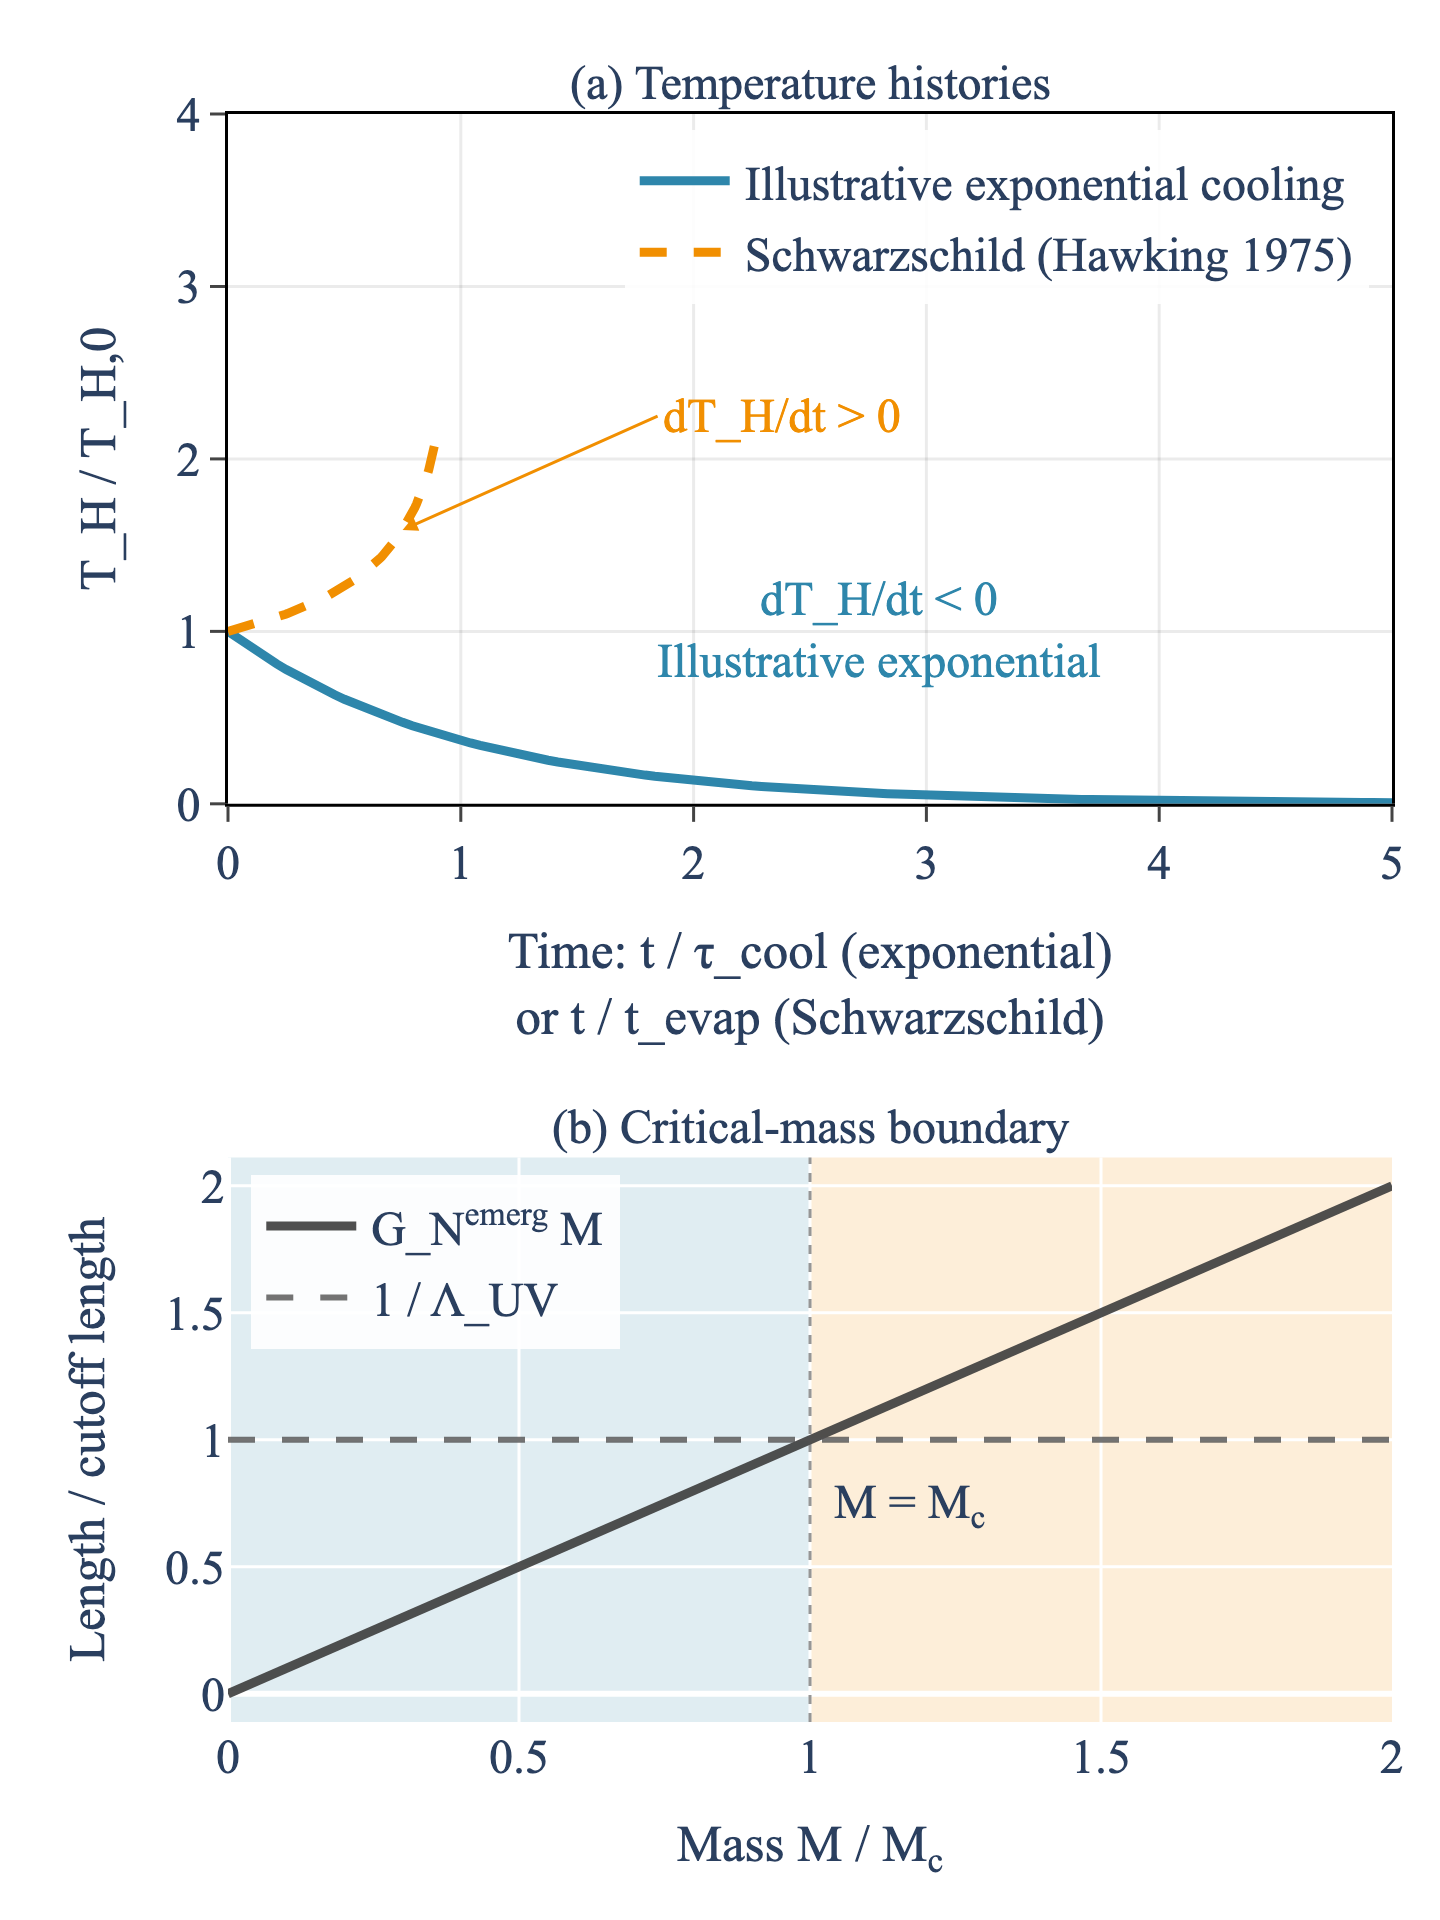
\includegraphics[width=0.8\textwidth]{figures/fig_T_H_evolution_regime_partition.png}
\caption{(a) Opposite temperature trends with separate normalized
clocks: $t/t_{\rm evap}$ for representative Schwarzschild evaporation
(amber, dashed), and $t/\tau_{\rm cool}$ for illustrative exponential
cooling (blue, solid). The exponential approaches zero asymptotically
and is distinct from the local affine nozzle result of
Balbinot \textit{et al.}~\cite{Balbinot2005PRD}.
(b) The emergent gravitational length $\GN M$ and cutoff length
$\Ladw^{-1}$, in cutoff-length units, coincide at $M = \Mc$.
Blue and amber shading indicate the branches below and above
this model boundary.}
\label{fig:regime-partition}
\end{figure*}

\section{Tracked-hypothesis bundle $H_{\rm RegimePartition}$}
\label{sec:hreg}

The load-bearing tracked hypothesis is the bundle
\begin{align}
H_{\rm RegimePartition}\,(b, p, \Thawk^{(0)}, &dT/dt|_{\rm evap}, \delta) := \nonumber \\
\text{conjunction of five fields:} \nonumber
\end{align}
\begin{description}
\item[\texttt{M\_c\_form\_consistent}:] $\Mc(p) > 0$.
\item[\texttt{T\_H0\_pos}:] $\Thawk^{(0)} > 0$.
\item[\texttt{evap\_dT\_dt\_above}:]
$b.M > \Mc(p) \;\Rightarrow\; 0 < dT/dt|_{\rm evap}$
(Schwarzschild heating sign per Hawking
1975~\cite{Hawking1975CMP}).
\item[\texttt{evap\_dT\_dt\_below}:]
$b.M < \Mc(p) \;\Rightarrow\; dT/dt|_{\rm evap} < 0$
(acoustic cooling sign per Balbinot
2005~\cite{Balbinot2005PRD} Eq.~Tsonic).
\item[\texttt{delta\_consistent\_with\_ansatz}:]
$\delta = (\aADW - 1) \Ladw$ (deep-research \S9 ansatz).
\end{description}

The rate $dT/dt|_{\rm evap}$ enters as an
\emph{externally-supplied real parameter}, not an existential.
This avoids the $\exists$-absorption anti-pattern: a witness
$dT/dt|_{\rm evap}$ supplied to the bundle must satisfy the
sign-claim consistent with the regime, rather than being existentially
discharged by any sign that happens to be present in the substrate.
The critical-mass positivity field is a consistency constraint implied
by parameter positivity; the branch-rate conditions remain supplied hypotheses.

The correctness-push theorem
\texttt{regime\_partition\_criterion} combines $H_{\rm RegimePartition}$
with the regime classifier:
\begin{align}
\text{classify}(b,p) = \texttt{Schwarzschild} &\;\Rightarrow\;
0 < dT/dt|_{\rm evap}, \nonumber \\
\text{classify}(b,p) = \texttt{ADWExtremality} &\;\Rightarrow\;
dT/dt|_{\rm evap} < 0.
\label{eq:regime-partition}
\end{align}
This theorem transports the two sign hypotheses through the mass
classifier. It does not derive an ADW evolution or the physical
location of its crossover. The local-profile criterion instead derives
slopes from an explicitly losing-mass trajectory and the affine nozzle
formula under its supplied short-time budget.

The substantive corollary
\texttt{delta\_ADW\_nonzero\_iff\_alpha\_ADW\_ne\_one} establishes
$\delta \neq 0 \;\Leftrightarrow\; \aADW \neq 1$, with the proof using
$\Ladw > 0$ from \texttt{ADWParams.Lambda\_pos} as a load-bearing field.

\section{The four laws in two regimes}
\label{sec:fourlaws}

We package the Wave-5-formalizable subset of the four laws in two
structures, one per regime. \texttt{FourLaws\_Schwarzschild} carries
\emph{three fields}: \texttt{firstLaw\_smarr}
(positivity of $\GN$ for the Smarr-identity coupling),
\texttt{secondLaw\_Schw} (\texttt{ADWSecondLaw} parameterized over
\texttt{entropy\_div}), and \texttt{evap\_dT\_dt\_positive}
(Schwarzschild heating sign $> 0$). The bundle is satisfied
consistently with the regime $b.M > \Mc(p)$.

\texttt{FourLaws\_ADWExtremality} carries the parallel three
fields, with two key modifications:
\texttt{firstLaw\_smarr\_with\_substrate} records positivity of
$\GN$ together with the ansatz $\delta = (\aADW - 1)\Ladw$; it does
not encode a differential first law or corrected Smarr identity.
The field
\texttt{evap\_dT\_dt\_negative} flips the evaporation-sign claim
(acoustic cooling sign $< 0$). The bundle is satisfied
consistently with the regime $b.M < \Mc(p)$.

The complete physical four-laws construction remains required.
The zeroth law ($\kappa$ constant on horizon) needs an actual horizon
and generator; the first law needs the thermodynamic variation and
charges; the second law needs an entropy/current construction linked
to that horizon. The third law needs an identified evolution and
quantitative affine-time control. The present structures do not supply
those constructions. In particular, the Balbinot $t \sim 1/T^3$
extrapolation does not establish acoustic Israel-strong preservation
(Section~\ref{sec:third}).

The Wave 5 \emph{gating theorem}
\texttt{four\_laws\_consistent\_with\_acoustic\_regime} combines the
classifier with the acoustic four-laws bundle and the
tracked-hypothesis structure. Its first conjunct returns the supplied
\texttt{FourLaws\_ADWExtremality} value; its second reads the supplied
negative rate under the mass classification. This is a conditional
consistency statement. It does not construct the physical laws or
identify an actual evaporation rate with the local nozzle derivative.

\section{Second law: Glorioso--Liu SK-EFT, no NEC}
\label{sec:sk-second}

The second law in both regimes is encoded via Glorioso and
Liu's theorem~\cite{GloriosoLiu2018} on dynamical KMS Z$_2$ symmetry
and unitarity (Im~$S_{\rm eff} \geq 0$) implying local
entropy-current monotonicity $\partial_\mu s^\mu \geq 0$,
\emph{without invoking pointwise NEC}. The
\texttt{ADWSecondLaw} Prop bundle takes the entropy-current
divergence as an externally-supplied real parameter
\texttt{entropy\_div} and records two fields:
\texttt{entropy\_divergence\_nonneg} ($0 \leq$ \texttt{entropy\_div},
the load-bearing Glorioso--Liu Eq.~(3.20) sign claim) and
\texttt{horizon\_area\_link\_consistent} ($0 < b.A$, the bundle's
horizon-area consistency witness). The KMS-Z$_2$ symmetry and
unitarity premises (Im~$S_{\rm eff} \geq 0$) of the Glorioso--Liu
derivation enter as substrate-side inputs that would become
substantive predicates on a formalized SK-EFT effective action; that
formalization is deferred to Phase 6e.

The Crossley--Glorioso--Liu constitutive
relations~\cite{CrossleyGloriosoLiu2017,GloriosoCrossleyLiu2017}
supply the SK-EFT framework. Applied to a BH horizon, this
replaces the classical Hawking 1971 area-non-decrease theorem (which
required pointwise NEC) with a local entropy-current monotonicity
that holds even when QFT operator-violations of pointwise NEC are
allowed in the bulk. Faulkner--Speranza~\cite{FaulknerSperanza2024}
derive the GSL algebraically from type-II crossed-product algebras;
Kirklin~\cite{Kirklin2024GSLAllOrders} extends to all orders in
perturbative gravity.

\section{Third law: BPS-conditional preservation, Kehle--Unger violation}
\label{sec:third}

Balbinot's $t \sim 1/T^3$ extrapolation suggests an infinite-time
zero-temperature limit in that nozzle model. It is not a controlled
late-time solution, and its time coordinate has not been identified
with horizon affine time. Israel-strong preservation for the physical
ADW branch therefore remains a separate construction. Kehle and
Unger~\cite{KehleUnger2022ThirdLaw} demonstrate that
charged-scalar-matter sectors can allow finite-time approach to
extremality. Reall~\cite{Reall2024ThirdLawBPS} provides the
BPS local mass-charge inequality under which the Israel form is
restored.

The module's \texttt{falsifier\_third\_law\_form}
(Section~\ref{sec:falsifiers}) proves that two supplied quantitative
approach-time predicates are incompatible: one is uniformly unbounded
as temperature tends to zero, and the other is bounded on a sufficiently
small positive-temperature interval. The theorem does not construct a
physical $\tau_{\rm approach}$ or prove either predicate for an ADW
trajectory. An affine-time model, its physical domain, and the relevant
matter assumptions remain part of the required third-law construction.

\section{Falsifier theorems}
\label{sec:falsifiers}

The Lean module gives four model-conditional checks on specified
profiles, supplied sign hypotheses, quantitative approach-time
predicates and the substrate-response ansatz. Physical use requires
matching those inputs to the ADW system. The checks derive
contradictions or sign constraints from their stated hypotheses and
the following mathematical results
(\texttt{T\_H\_acoustic\_evolution\_strict\_decreasing} for falsifier
1, \texttt{H\_RegimePartition.evap\_dT\_dt\_above} for falsifier 2,
the $\min$ argument over the two-sided thresholds for falsifier 3,
the substrate's $\Ladw > 0$ field for falsifier 4).

\begin{enumerate}
\item \textbf{Acoustic-decay form falsifier}
  (\texttt{falsifier\_acoustic\_decay\_form}): given a candidate
  $\Thawk^{\rm alt}(t)$ that matches the chosen exponential
  $\Thawk^{\rm acoustic}(t_1)$ at time $t_1$ AND fails to strictly
  decrease by time $t_2$ ($\Thawk^{\rm alt}(t_1) \leq
  \Thawk^{\rm alt}(t_2)$), the candidate must DISAGREE with
  $\Thawk^{\rm acoustic}(t_2)$. The proof uses the strict-decreasing
  theorem to derive a contradiction.
\item \textbf{Schwarzschild-heating sign falsifier}
  (\texttt{falsifier\_schwarzschild\_heating}): given the
  $H_{\rm RegimePartition}$ bundle and a Schwarzschild-regime
  classification, an observed non-positive $dT/dt$ contradicts the
  bundle's \texttt{evap\_dT\_dt\_above} sign claim
  (Hawking 1975~\cite{Hawking1975CMP}). Conclusion is \texttt{False}.
\item \textbf{Third-law-form falsifier}
  (\texttt{falsifier\_third\_law\_form}): given a strong-Israel
  predicate (approach time unbounded as $\varepsilon \to 0$) and a
  Kehle--Unger predicate (approach time bounded above for small
  enough $\varepsilon$), the two are mutually inconsistent; the proof
  takes $\varepsilon = \min(\varepsilon_0, \varepsilon_{\rm th})$
  where both predicates apply and derives a contradiction. Conclusion
  is \texttt{False}.
\item \textbf{$\aADW$-dependence falsifier}
  (\texttt{falsifier\_alpha\_ADW\_dependence}; renamed from the
  initial-ship name \texttt{falsifier\_chi\_vest\_dependence} per a
  Stage-13 finding flagging that the deep-research \S9 ansatz
  $\dADW = (\aADW - 1)\Ladw$ depends on $\aADW$ and $\Ladw$, not
  directly on $\xivest$). The conclusion $0 < (\aADW - 1)\Ladw$ uses
  both $\aADW > 1$ and the substrate's $\Ladw > 0$ field; a
  measurement of opposite sign falsifies the ansatz.
\end{enumerate}

\section{Lean Formalization}
\label{sec:lean}

The module \texttt{BHThermodynamicsFourLaws.lean}
ships \bhThermoTotal{} theorems, \sorrycount{} sorry, 0 new axioms.
Verification via \texttt{\#print axioms} on six substantive theorems
(\texttt{regime\_partition\_criterion},
\texttt{four\_laws\_consistent\_with\_acoustic\_regime},
\texttt{falsifier\_acoustic\_decay\_form},
\texttt{falsifier\_schwarzschild\_heating},
\texttt{falsifier\_third\_law\_form},
\texttt{wave3\_bridge\_kaul\_majumdar\_at\_e\_squared\_anchor})
shows dependency only on $\{$\texttt{propext}, \texttt{Classical.choice},
\texttt{Quot.sound}$\}$.

The structures expose their hypotheses: the evaporation rate and
entropy-current divergence are supplied real parameters; positivity
of $\GN$ follows from the parameter carrier. The acoustic consistency
theorem returns its supplied mechanics structure together with a sign
read from the regime hypothesis. The local-profile theorem separately
uses derivatives of specified functions. These statements must be read
with those carriers; kernel purity alone does not establish physical
thermodynamic laws. No zeroth- or third-law field is present in the two
\texttt{FourLaws\_*} structures, and the complete physical construction
remains required.

\section{Cross-wave compatibility}
\label{sec:cross}

\textbf{Wave 1} (\texttt{LinearizedEFE.G\_N\_emerg}): the first-law
coupling $1/(8\pi \GN)$ in both \texttt{FourLaws\_*} bundles uses
Wave 1's $\GN$ evaluated at substrate parameters. The bridge
\texttt{wave1\_bridge\_G\_N\_emerg\_pos} records that positivity of
$\GN$ propagates through to both regime branches.

\textbf{Wave 2} ($c_{\rm GW} = c \cdot \sqrt{\xivest}$): the
acoustic substrate inherits the metric-channel speed via
$\kappa$ dependence on $\xivest$.

\textbf{Horizon-entropy connection.} The theorem
\texttt{wave3\_bridge\_\allowbreak kaul\_majumdar\_\allowbreak at\_e\_squared\_anchor}
calls \texttt{BHEntropyMicroscopic.kaulMajumdarS} at
$A = 4\,G_N\,e^2$, giving $S = e^2 - 3 > 0$ for positive $G_N$.
This is a concrete entropy-value statement. It contains no temperature
or evolution argument identifying that area with a physical
zero-temperature endpoint. Establishing that identification and the
appropriate Nernst limit remains required; positivity at a supplied
area does not itself prove either Nernst law.

\section{Novelty Flags}
\label{sec:novelty}

\textbf{Project-original}:
\begin{itemize}
\item The ADW-substrate-specific critical mass
  $\Mc(\aADW, \Ladw, \Nf) = (\Nf \Ladw) / (12\pi \aADW)$
  ansatz is project-original.
\item The cross-regime gluing (Schwarzschild for $b.M > \Mc$,
  acoustic for $b.M < \Mc$) is project-conjecture; no published
  paper proposes a single emergent-gravity BH with this regime
  structure.
\item The $\dADW = (\aADW - 1)\Ladw$ substrate-response coefficient
  ansatz is original (deep-research \S9).
\end{itemize}

\textbf{Primary-source-grounded}:
\begin{itemize}
\item Schwarzschild branch: Hawking 1975~\cite{Hawking1975CMP}.
\item Local nozzle cooling: Balbinot et al.~\cite{Balbinot2005PRD},
  Eq.~(Tsonic). The chosen exponential is a separate illustrative
  profile; physical ADW branch matching remains required.
\item Second law: Glorioso--Liu~\cite{GloriosoLiu2018}
  (no NEC needed).
\item Third law conditional: Israel 1986 (strong form) /
  Kehle--Unger~\cite{KehleUnger2022ThirdLaw} /
  Reall~\cite{Reall2024ThirdLawBPS}.
\end{itemize}

\section{Conclusions}
\label{sec:conclusions}

The formalized classifier partitions a proposed ADW mass scale and
transports supplied evaporation signs. The separate local-profile
criterion derives heating for a differentiable, positive, losing-mass
Schwarzschild trajectory and cooling for the affine nozzle model under
its explicit short-time assumptions. The exponential shown in the
figure is illustrative. Physical ADW branch selection, a controlled
cross-cutoff evolution and a late-time endpoint do not follow from
these conditional and local results.

The Lean module ships \bhThermoTotal{} theorems, \sorrycount{} sorry,
0 new axioms; the load-bearing tracked hypothesis encodes the
sign claims as constraints on an externally-supplied evaporation
rate, avoiding the $\exists$-absorption anti-pattern. The
substrate-response coefficient ansatz $\dADW = (\aADW - 1)\Ladw$
provides four falsifiability tests for any candidate ADW substrate.

The original physical objective remains the full four-laws
construction for an emergent ADW black hole. It requires a microscopic
action and selected background, horizon/charge/entropy observables,
energy and entropy balances, calibrated mass and cutoff matching,
and controlled dynamics with quantitative remainder and affine-time
bounds. The present classifier, local profiles and conditional
structures supply supporting mathematics; they do not complete that
objective.
% Publication BUILD obligations remain OPEN in
% docs/audits/2026-10-17-publication-substance-construction/REPAIR_DISPOSITION_MAP.md.

% Source-acquisition and review history is retained in the publication review record.

\begin{thebibliography}{99}

\bibitem{Hawking1975CMP}
S.~W. Hawking,
\textit{Particle creation by black holes},
Commun. Math. Phys. \textbf{43}, 199 (1975).
DOI: 10.1007/BF02345020.

\bibitem{Balbinot2005PRD}
R.~Balbinot, S.~Fagnocchi, A.~Fabbri,
\textit{Quantum Effects in Acoustic Black Holes: the Backreaction},
Phys. Rev. D \textbf{71}, 064019 (2005). arXiv:gr-qc/0405098.

\bibitem{JacobsonVolovik1998}
T.~A.~Jacobson and G.~E.~Volovik,
\textit{Event horizons and ergoregions in $^3$He},
Phys. Rev. D \textbf{58}, 064021 (1998). arXiv:cond-mat/9801308.

\bibitem{JacobsonKoike2002}
T.~A.~Jacobson and T.~Koike,
\textit{Black hole and baby universe in a thin film of $^3$He-A},
in M.~Novello, M.~Visser, G.~Volovik (eds.), \textit{Artificial Black
Holes} (World Scientific, 2002). arXiv:cond-mat/0205174.

%% Removed Volovik2003BraneBH — not cited in current paper prose.
%% Retained in CITATION_REGISTRY for future cross-reference.

\bibitem{KehleUnger2022ThirdLaw}
C.~Kehle, R.~Unger,
\textit{Gravitational collapse to extremal black holes and the
third law of black hole thermodynamics},
J. Eur. Math. Soc. (2025), DOI 10.4171/JEMS/1591. arXiv:2211.15742.

\bibitem{Reall2024ThirdLawBPS}
H.~S.~Reall,
\textit{A third law of black hole mechanics for supersymmetric black
holes and a quasi-local mass-charge inequality},
Phys. Rev. D \textbf{110}, 124059 (2024). arXiv:2410.11956.

\bibitem{GloriosoLiu2018}
P.~Glorioso, H.~Liu,
\textit{The second law of thermodynamics from symmetry and unitarity},
arXiv:1612.07705.

\bibitem{CrossleyGloriosoLiu2017}
M.~Crossley, P.~Glorioso, H.~Liu,
\textit{Effective field theory of dissipative fluids},
JHEP \textbf{09}, 095 (2017). arXiv:1511.03646.

\bibitem{GloriosoCrossleyLiu2017}
P.~Glorioso, M.~Crossley, H.~Liu,
\textit{Effective field theory of dissipative fluids II:
classical limit, dynamical KMS symmetry and entropy current},
JHEP \textbf{09}, 096 (2017). arXiv:1701.07817.

%% Removed HawkingHorowitzRoss1995 — not cited in current paper prose.
%% Retained in CITATION_REGISTRY for future cross-reference.

\bibitem{FaulknerSperanza2024}
T.~Faulkner, A.~Speranza,
\textit{Gravitational algebras and the generalized second law},
arXiv:2405.00847.

\bibitem{Kirklin2024GSLAllOrders}
J.~Kirklin,
\textit{Generalised second law beyond the semiclassical regime},
JHEP \textbf{07}, 192 (2025). arXiv:2412.01903.

%% Removed StrengtheningPost2026 (internal project memo, not externally citable).
%% The four-pattern anti-vacuity audit is now described inline in §sec:lean.

\end{thebibliography}

\end{document}
